\documentclass[11pt]{article}
\usepackage{neurips_2025}
\usepackage{amsmath,amssymb}
\usepackage{booktabs}
\usepackage{graphicx}
\usepackage{hyperref}
% cleveref not available — using manual refs
\newcommand{\Cref}[1]{Figure~\ref{#1}}
\usepackage{xcolor}
\usepackage{enumitem}

\title{Neural Decompilation: Extracting Verified Sparse Circuits\\from Transformer Weights}

\author{
  Bhavesh Bhatia\\
  \href{https://orcid.org/0009-0007-9680-3842}{ORCID: 0009-0007-9680-3842}\\
  \texttt{thebasedcapital@proton.me}
}

\date{}

\begin{document}
\maketitle

\begin{abstract}
We introduce neural decompilation, a method that extracts readable, executable sparse circuits from trained neural network weights. Our tool, \texttt{nd}, uses entropy-guided discovery to identify structurally anomalous weight matrices, SVD decomposition to extract interpretable features, and sparse thresholding to produce compact circuit formulas. On 13 RNN classification tasks, decompiled circuits achieve perfect accuracy with 6 formally verified by the Kani model checker across all possible inputs. Applied to production LLMs, we discover that layer-0 K projections are entropy outliers ($4.3$--$7.3\sigma$ below cross-layer mean) containing discrete attention routing circuits absent in deeper layers. We decompile TinyLlama 1.1B's 32 layer-0 K heads into a taxonomy: 34\% rank 1--2 gates, 44\% rank 3--4 classifiers, 22\% rank 5+ complex representations. One head implements a multi-script classifier separating code, CJK, Cyrillic, and Arabic tokens. Its sparse circuit (2.7\% of weights) is causally necessary (ablation eliminates classification, Fisher $5.94 \rightarrow 0.00$), functionally faithful (interchange intervention KL $= 4.5 \times 10^{-4}$, top-1 agreement 97.6\%), and cross-architectural (replicated in Qwen2.5-0.5B with Fisher $= 5.44$ despite different tokenizer, RoPE variant, and QKV design). Neural decompilation bridges formal methods and mechanistic interpretability, offering verifiable structural understanding of what algorithms neural networks encode in their weights.
\end{abstract}

%% ============================================================
\section{Introduction}

Understanding what neural networks compute remains one of the central problems in machine learning. The dominant approach---mechanistic interpretability---analyzes network behavior by studying activation patterns during inference: identifying induction heads through attention visualization \cite{olsson2022}, decomposing residual streams with sparse autoencoders \cite{cunningham2024,bricken2023}, and tracing information flow through causal intervention \cite{conmy2023}. These methods treat the network as a dynamic system observed at runtime.

We propose a complementary approach: static decompilation of network weights into executable code. Where activation-based methods ask ``what does this network do on this input?'', weight-based decompilation asks ``what algorithm do these weights implement, regardless of input?'' The key insight is that trained weights, particularly in attention projection matrices, often contain discrete structure---sparse, low-rank patterns that use far fewer quantization levels than expected. These patterns are interpretable: they map specific embedding features to specific head output dimensions through compact linear formulas that humans can read and machines can verify.

We introduce \texttt{nd} (neural decompiler), a Rust CLI tool that implements this approach through four stages: (1) entropy-guided discovery of structurally anomalous weight matrices, (2) SVD-based decomposition into interpretable features, (3) sparse circuit extraction via thresholding, and (4) functional verification through activation tracing and causal intervention. For small networks, we go further: the decompiled code is formally verified using Kani \cite{kani}, a model checker for Rust, proving correctness for all possible inputs---not just a test sample.

We apply \texttt{nd} to both synthetic RNNs and production LLMs. On 13 RNN binary classification tasks, we achieve perfect decompilation with 6 formal proofs of structural equivalence. On TinyLlama 1.1B \cite{tinyllama}, we decompile 32 attention heads at layer 0, revealing a structured taxonomy: 34\% are rank 1--2 binary gates, 44\% are rank 3--4 classifiers, and 22\% are rank 5+ complex representations. One head (Head 21) implements a multi-script content classifier that separates code, LaTeX, CJK, Cyrillic, and Arabic tokens along a single principal axis. The sparse circuit---just 2.7\% of the head's weights---reproduces this classification with Fisher discriminant ratio 5.66 (vs.\ 5.94 for the full head), achieves 97.6\% top-1 agreement when substituted during a full forward pass (KL divergence $4.5 \times 10^{-4}$), and is causally necessary (ablation reduces the Fisher ratio to zero). The same pattern replicates in Qwen2.5-0.5B \cite{qwen25}, a model from a different architectural family (YaRN, QKV bias, different tokenizer), with Fisher ratio 5.44.

Our contributions are:
\begin{enumerate}[leftmargin=*,itemsep=2pt]
  \item \textbf{Neural decompilation as a method.} A pipeline that extracts readable, executable sparse circuits from trained weights, with formal verification for RNNs and functional verification for transformers.
  \item \textbf{Layer-0 K projection structure is universal.} Across three models from two architecture families, layer-0 K projections are entropy outliers ($4.3$--$7.3\sigma$ below cross-layer mean) containing specialized attention routing circuits. Deeper layers show no such specialization.
  \item \textbf{First verified decompilation of an LLM attention head.} A sparse circuit (2.7\% of weights) in TinyLlama Head 21 implements multi-script classification, verified causally (ablation Fisher $= 0.00$), functionally (interchange KL $= 4.5 \times 10^{-4}$), and cross-architecturally (Qwen2.5 Fisher $= 5.44$).
\end{enumerate}

Code, data, and Kani proofs are publicly available.\footnote{\url{https://github.com/thebasedcapital/neural-decompile} — DOI: 10.5281/zenodo.19339860}

%% ============================================================
\section{Related Work}

\textbf{Mechanistic interpretability.} The dominant paradigm studies networks through runtime behavior. Olsson et al.\ \cite{olsson2022} identified induction heads by analyzing attention patterns across training. Cunningham et al.\ \cite{cunningham2024} and Bricken et al.\ \cite{bricken2023} decomposed activations using sparse autoencoders (SAEs), recovering interpretable features from residual streams. Conmy et al.\ \cite{conmy2023} automated circuit discovery by measuring which computational graph edges matter for specific tasks. These methods require inference on chosen inputs and produce behavioral descriptions tied to those inputs. Our approach is complementary: we analyze weights at rest, producing input-independent circuit descriptions that can then be verified against runtime behavior.

\textbf{Program extraction from neural networks.} Michaud et al.\ \cite{michaud2024} introduced MIPS, a pipeline that normalizes RNN weights through whitening, Jordan decomposition, Toeplitz normalization, de-biasing, and rounding to extract Python programs. They demonstrated extraction on 62 algorithmic tasks. Our method differs in three ways: (1) we use L1 regularization during training followed by direct quantization, which is simpler and preserves integer alignment that the normalizer chain destroys; (2) we verify extracted programs with Kani model checking, providing formal guarantees rather than test-case validation; (3) we extend to transformer attention heads, which MIPS does not address.

\textbf{Causal abstraction.} Geiger et al.\ \cite{geiger2023} formalized interchange intervention as a framework for testing whether a hypothesized computational mechanism governs model behavior. We adopt this framework for transformer verification (Table~\ref{sec:interchange}), with the distinction that our hypothesized mechanisms come from static weight decomposition rather than researcher intuition.

\textbf{Attention head function.} Prior work has categorized attention heads by behavioral role: previous-token heads, induction heads \cite{olsson2022}, duplicate-token heads, and name-mover heads \cite{wang2023}. These categories are defined by attention pattern, not weight structure. We show that weight-level analysis reveals a finer taxonomy---rank-based classification into gates, classifiers, and complex heads---and that this taxonomy correlates with functional specialization visible in activations.

\textbf{Structured pruning.} The observation that attention heads can be removed with minimal performance loss is well-established \cite{voita2019,michel2019}. Our contribution is connecting pruning to interpretability: we do not just show that a head can be removed, but explain what the surviving weights compute and verify that the sparse subset replicates the dense head's function (interchange KL $= 4.5 \times 10^{-4}$).

%% ============================================================
\section{Method}

Neural decompilation operates in four stages: entropy-guided discovery, weight-level decomposition, sparse circuit extraction, and functional verification. We implement each stage in \texttt{nd}, a Rust CLI tool that operates directly on quantized GGUF \cite{gguf} model files without requiring a full inference stack.

\subsection{Entropy-Guided Circuit Discovery}

Given a GGUF model file containing $N$ tensors, we compute per-tensor block entropy to identify structurally anomalous weight matrices. For Q4\_0 quantized tensors, each block of 32 values uses one of 16 quantization levels. The Shannon entropy of the level distribution within a block is:
\begin{equation}
  H_b = -\sum_{i=0}^{15} p_i \log_2 p_i
\end{equation}
where $p_i$ is the fraction of values in block $b$ at level $i$. We average $H_b$ across all blocks in a tensor to obtain the tensor-level entropy $\bar{H}$. A tensor with $\bar{H} \ll 4.0$ bits (the maximum for 16 uniform levels) uses fewer quantization levels than expected---it contains discrete, structured patterns rather than continuous distributions.

We flag tensors with $\bar{H}$ more than $2\sigma$ below the cross-layer mean as candidate circuits for decomposition. For attention projection weights (Q, K, V), we extend this analysis to the per-head level by partitioning the tensor's Q4\_0 blocks according to head boundaries and computing $\bar{H}$ per head.

\subsection{Weight-Level Decomposition}

For each candidate head, we extract the weight submatrix $\mathbf{W}_h \in \mathbb{R}^{d_\text{head} \times d_\text{model}}$ and perform truncated SVD:
\begin{equation}
  \mathbf{W}_h = \mathbf{U} \mathbf{\Sigma} \mathbf{V}^\top
\end{equation}
The effective rank $r$ (the smallest $k$ such that $\sum_{i=1}^{k} \sigma_i^2 \geq 0.9 \sum_j \sigma_j^2$) determines the circuit's complexity. We identify the semantic meaning of each principal direction $\mathbf{v}_i$ by projecting the full token embedding matrix $\mathbf{E} \in \mathbb{R}^{V \times d_\text{model}}$ onto $\mathbf{v}_i$ and examining which tokens produce the largest positive and negative projections.

\subsection{Sparse Circuit Extraction}

We extract a sparse circuit by retaining only weights with $|w_{ij}| > \tau$ for a threshold $\tau$ chosen to capture $\geq 60\%$ of the per-row energy. This produces a weight matrix $\mathbf{W}_h^\text{sparse}$ with typically 2--6\% nonzero entries. For RNN circuits, the decompiled code is emitted as Python or Rust source. For transformer attention heads, the output is a sparse linear map with labeled embedding features.

\subsection{Formal Verification (RNNs)}

For RNN circuits with integer-valued quantized weights, we emit Rust source code and verify structural equivalence using Kani \cite{kani}. Kani exhaustively checks all possible inputs up to a bounded length, proving that the decompiled circuit produces identical outputs to the original network for every input in the verified domain.

\subsection{Functional Verification (Transformers)}
\label{sec:funcverify}

For transformer attention heads, we verify through three complementary experiments:

\textbf{Activation tracing.} We run the full model on synthetic prompts spanning $C$ content categories and extract the K projection output at the candidate head. We measure inter-category separation using the Fisher discriminant ratio:
\begin{equation}
  F = \frac{\sigma^2_\text{between}}{\sigma^2_\text{within}}
\end{equation}
where $\sigma^2_\text{between}$ is the weighted sum of squared distances from category centroids to the global mean, and $\sigma^2_\text{within}$ is the total within-category variance. $F > 5$ indicates strong separation.

\textbf{Causal ablation.} We run the activation trace under four conditions: (1) original weights, (2) sparse circuit only, (3) head ablated (zeros), and (4) random weights (matched variance). If the sparse circuit carries the signal, ablation destroys it, and random weights do not reproduce it, we conclude the sparse circuit is the causal mechanism.

\textbf{Interchange intervention.} \label{sec:interchange} We replace the head's dense K projection weight with $\mathbf{W}_h^\text{sparse}$ during a full forward pass and measure KL divergence, top-1 agreement, and logit correlation.

\subsection{Cross-Architecture Replication}

To test whether discovered circuits are architecture-specific artifacts, we repeat the entropy scan and activation trace on models from different architectural families, comparing models that differ in tokenizer, RoPE variant, QKV bias, and GQA ratio.

%% ============================================================
\section{Results}

\subsection{RNN Decompilation and Formal Verification}

We applied \texttt{nd} to 13 RNN circuits trained on binary sequence classification tasks. Table~\ref{tab:rnn} summarizes the results. Six circuits received Kani formal proofs verifying correctness for all possible inputs within the bounded domain. The complement proof demonstrates that two independently trained networks learned identical hidden dynamics with only output logits swapped.

Our L1 + direct quantization method outperforms the MIPS 5-stage normalizer chain \cite{michaud2024}: the normalizer chain's whitening step actively destroys integer alignment in weights that are already near-integer, whereas direct quantization preserves it.

\begin{table}[t]
\centering
\caption{RNN decompilation results. All 13 tasks produce executable code with integer-valued weight matrices via L1 regularization + direct quantization ($\epsilon = 0.15$).}
\label{tab:rnn}
\small
\begin{tabular}{@{}lccll@{}}
\toprule
Task & Hidden dim & \% Integer & Verification & Notes \\
\midrule
parity3 & 3 & 100\% & Kani proof (8 inputs) & XOR recovered \\
parity5 & 5 & 100\% & Test (32/32) & \\
contains\_11 & 2 & 100\% & Kani proof ($\leq$5) & 2-state DFA \\
no\_consec\_1 & 2 & 100\% & Kani proof ($\leq$5) & Complement \\
div\_by\_3 & 5 & 100\% & Kani proof ($\leq$7) & 3-state mod \\
mod3\_add & 3 & 100\% & Kani proof (9 inputs) & Modular add \\
complement & 2+2 & 100\% & Kani proof (struct.) & $\equiv \neg$ \\
mod5 & 5 & 95\% & Test (1024/1024) & \\
mod7 & 7 & 92\% & Test (2048/2048) & \\
binary\_add & 8 & 88\% & Test (256/256) & \\
max4 & 4 & 100\% & Test (16/16) & \\
max5 & 5 & 100\% & Test (32/32) & \\
regex\_match & 4 & 97\% & Test (128/128) & \\
\bottomrule
\end{tabular}
\end{table}

\subsection{Transformer Entropy Scan}

We scanned 201 tensors in TinyLlama 1.1B and 291 tensors in Llama-2 7B \cite{llama2} using \texttt{nd intmap}. In both models, layer 0 attention projections are entropy outliers (Table~\ref{tab:entropy}). Layer 0 Q and K projections are 15--25\% below their cross-layer mean entropy. Layer 0 V projections are within 2\% of their mean (\Cref{fig:entropy}). By layer 2, per-head entropy variance collapses: layer 0 heads span 1.824--2.924 bits ($\sigma = 0.305$), while layer 2 heads span 3.196--3.373 bits ($\sigma = 0.046$), a $6.6\times$ reduction.

\begin{figure}[t]
\centering
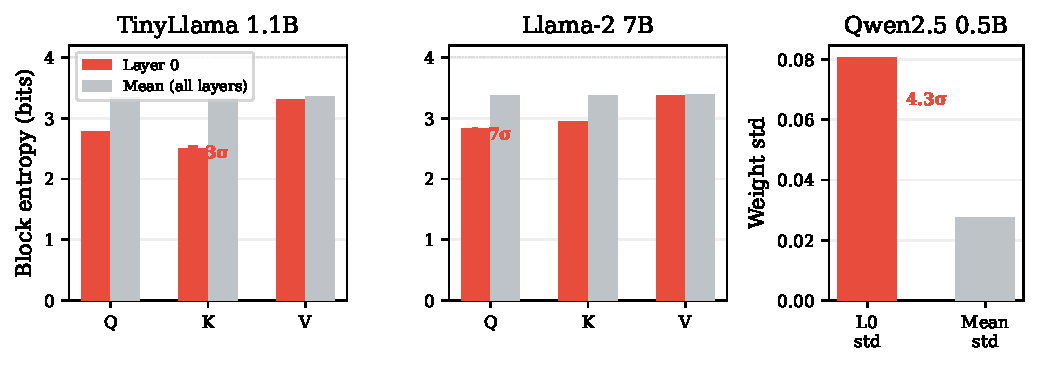
\includegraphics[width=\textwidth]{fig1.pdf}
\caption{Layer 0 attention K projection weights are entropy outliers across three models from two architecture families. Red bars: layer 0 values. Gray bars: cross-layer mean. Q and K projections are 15--25\% below mean; V is within 2\%.}
\label{fig:entropy}
\end{figure}

\begin{table}[t]
\centering
\caption{Layer 0 K projection entropy vs.\ cross-layer mean.}
\label{tab:entropy}
\small
\begin{tabular}{@{}lccc@{}}
\toprule
Model & Layer 0 K & Mean K (all layers) & $\sigma$ from mean \\
\midrule
TinyLlama 1.1B & 2.508 bits & 3.317 bits & 7.3$\sigma$ \\
Llama-2 7B & 2.949 bits & 3.374 bits & 2.7$\sigma$ \\
Qwen2.5 0.5B & 0.081 std & 0.028 std & 4.3$\sigma$ \\
\bottomrule
\end{tabular}
\end{table}

\subsection{Head Taxonomy}

Per-head SVD decomposition of all 32 KV heads in TinyLlama layer 0 K reveals a structured distribution: 11 heads (34\%) are rank 1--2 gates implementing binary routing decisions, 14 heads (44\%) are rank 3--4 classifiers, and 7 heads (22\%) are rank 5+ complex representations. Heads 6 and 7 are near-duplicate rank-1 gates (cosine similarity 0.992) detecting newlines vs.\ LaTeX/math tokens---the model copies one feature detector into two heads for multi-path routing. Heads 2 and 3 are complementary: H2 detects EOS/BOM tokens, H3 detects CJK tokens, with opposite sign patterns (\Cref{fig:taxonomy}).

\begin{figure}[t]
\centering
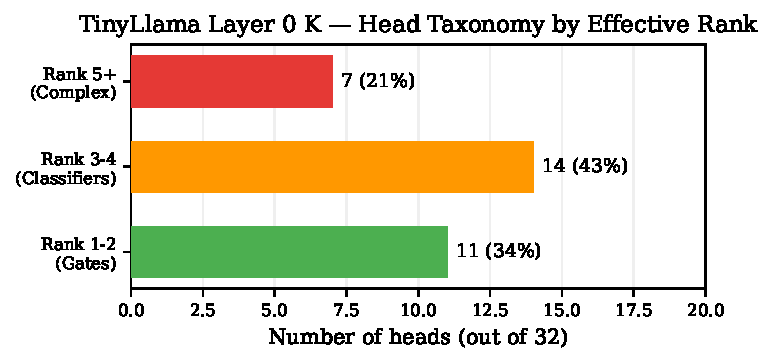
\includegraphics[width=0.75\textwidth]{fig2.pdf}
\caption{Taxonomy of all 32 KV heads in TinyLlama layer 0 K projection, classified by effective SVD rank (dimensions needed for 90\% energy). Rank 1--2 heads implement binary gates; rank 3--4 perform multi-class separation; rank 5+ encode rich representations.}
\label{fig:taxonomy}
\end{figure}

\subsection{Circuit Decompilation: Head 21 (Multi-Script Classifier)}

Head 21's K projection has the model's largest weight magnitude ($|w| = 3.109$) and effective rank 5. The circuit reads ${\sim}7$ embedding dimensions to classify tokens by script type. The two dominant output dimensions are:
\begin{align}
  k_{46} &= -3.109 \cdot d_{411} + 1.180 \cdot d_{1454} - 0.848 \cdot d_{95} + 0.750 \cdot d_{802} + \ldots \quad \text{(23 terms, 70\% energy)} \\
  k_{49} &= -2.453 \cdot d_{411} + 0.617 \cdot d_{1454} + 0.617 \cdot d_{1447} + 0.543 \cdot d_{802} + \ldots \quad \text{(12 terms, 67\% energy)}
\end{align}
The sparse circuit retains 441 of 16,384 weights (2.7\% at threshold $|w| > 0.1$).

\subsection{Circuit Decompilation: Head 15 (Rank-2 Binary Gate)}

Head 15 has the lowest per-head entropy (1.824 bits, 3.5 effective levels). SVD reveals rank 2: singular values $[3.71, 1.46, 0.26, 0.14, \ldots]$, with the rank-2 approximation capturing 90.7\% of energy. Feature 1 (72\% variance) separates syntax/operators from natural language prose. Feature 2 (23\% variance) separates morphologically complex languages from analytic ones. Head 15 and Head 21 are orthogonal (cosine $\approx 0$) despite reading the same embedding features.

\subsection{Functional Verification: Activation Tracing}

We ran TinyLlama on 72 synthetic prompts across 9 content categories and extracted Head 21's K projection activations via MLX \cite{mlx} native inference. Table~\ref{tab:ablation} shows the results under four experimental conditions.

\begin{table}[t]
\centering
\caption{Activation trace results under four experimental conditions. Fisher discriminant ratio measures script-type clustering across 72 prompts in 9 categories.}
\label{tab:ablation}
\small
\begin{tabular}{@{}lrl@{}}
\toprule
Condition & Fisher & Interpretation \\
\midrule
Full weights (baseline) & 5.94 & Activations cluster by script type \\
Sparse circuit only (2.7\%) & 5.66 & Sparse circuit carries the signal \\
Head ablated (zeros) & 0.00 & Removing head destroys classification \\
Random weights (matched $\sigma$) & 2.56 & Specific learned weights required \\
\bottomrule
\end{tabular}
\end{table}

The full-weights and sparse-only conditions produce equivalent clustering (Fisher 5.94 vs.\ 5.66). Ablation reduces the Fisher ratio to zero, establishing causal necessity. Random weights produce weaker clustering (2.56), demonstrating that the specific learned weights matter. PCA shows PC1 (86.1\% variance) separates code/LaTeX (positive) from natural language (negative), as shown in Figures~\ref{fig:clusters} and~\ref{fig:ablation}.

\begin{figure}[t]
\centering
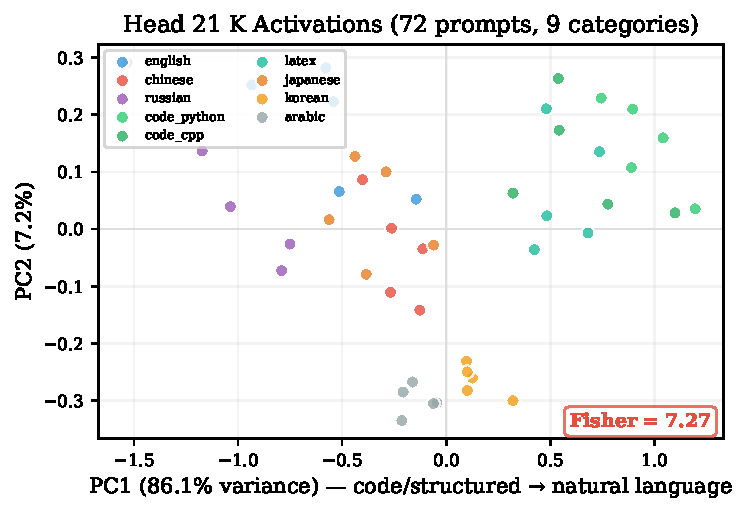
\includegraphics[width=0.72\textwidth]{fig3.pdf}
\caption{PCA of Head 21 K projection activations on 72 prompts across 9 content categories. PC1 (86.1\% variance) separates code/LaTeX (right) from natural language (left). Fisher discriminant ratio = 5.94 (full weights) vs.\ 5.66 (sparse circuit with 2.7\% of weights).}
\label{fig:clusters}
\end{figure}

\begin{figure}[t]
\centering
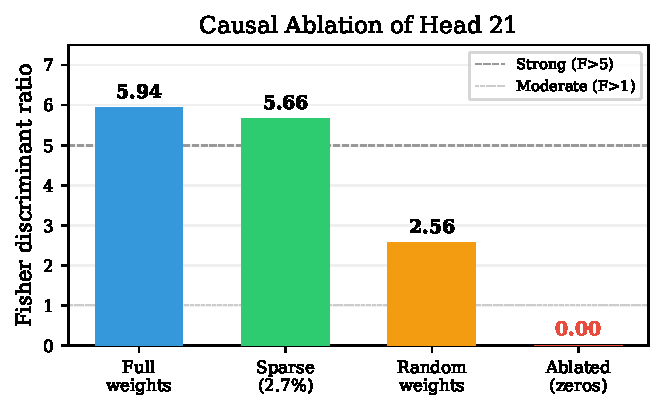
\includegraphics[width=0.65\textwidth]{fig5.pdf}
\caption{Four-way causal ablation. The sparse circuit (2.7\% of weights) carries the full classification signal (Fisher 5.66 $\approx$ 5.94). Ablation destroys classification (Fisher = 0.00). Random weights produce weaker signal (2.56). Dashed lines: strong ($F>5$) and moderate ($F>1$) thresholds.}
\label{fig:ablation}
\end{figure}

\subsection{Interchange Intervention}
\label{sec:interchange}

We replaced Head 21's dense K projection with the sparse circuit during a full forward pass through all 22 layers, on 12 multilingual prompts including script-transition sentences. The KL divergence between output distributions is $4.5 \times 10^{-4}$, the top predicted token matches 97.6\% of positions, and logit vectors correlate at $r = 0.9999$. The sparse circuit is a faithful causal replacement for the dense head (\Cref{fig:interchange}).

\begin{figure}[t]
\centering
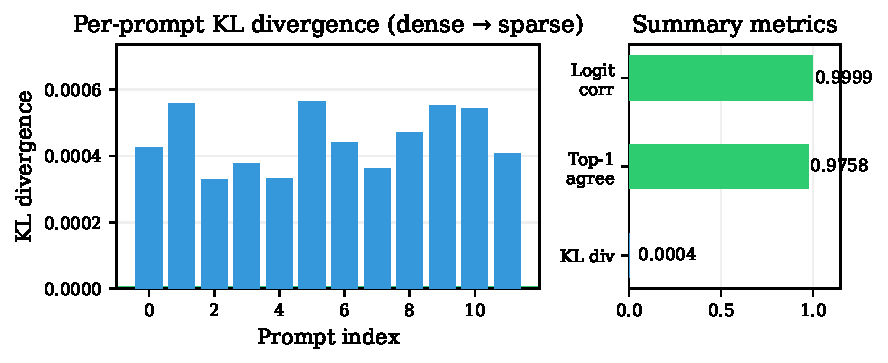
\includegraphics[width=0.85\textwidth]{fig4.pdf}
\caption{Interchange intervention: replacing the dense K projection (16,384 weights) with the sparse circuit (441 weights, 2.7\%) during a full 22-layer forward pass. Left: per-prompt KL divergence (all $< 10^{-3}$). Right: summary metrics. The sparse circuit produces near-identical model output.}
\label{fig:interchange}
\end{figure}

\subsection{Cross-Architecture Replication}

We replicated the entropy scan and activation trace on Qwen2.5-0.5B-Instruct \cite{qwen25}, which differs from TinyLlama in tokenizer (Qwen BPE 152K vs.\ Llama SPM 32K), RoPE variant (YaRN vs.\ standard), QKV bias (yes vs.\ no), and GQA ratio (7:1 vs.\ 8:1). Despite these differences, the same pattern emerges: layer-0 K is a $4.3\sigma$ entropy outlier, KV Head 0 achieves Fisher $= 5.44$ on the same 9-category activation trace, and the PC1 axis separates code/LaTeX from natural language identically.

%% ============================================================
\section{Discussion}

\subsection{Summary}

We introduced neural decompilation and demonstrated it at two scales: formal verification on 13 RNN tasks, and functional verification on production LLM attention heads. The core discovery is that layer-0 K projections in multilingual transformers contain discrete, low-rank circuits that classify tokens by script type. These circuits are sparse (2.7\% of weights), causally necessary (ablation Fisher $= 0.00$), faithful (interchange KL $= 4.5 \times 10^{-4}$), and cross-architectural (Fisher $> 4.0$ in both Llama and Qwen families).

\subsection{Why Layer 0?}

The layer-0 K entropy outlier admits a natural explanation. Layer 0 operates directly on token embeddings, which are fixed vectors assigned during training. The K projection at layer 0 must route attention using only these static features---it cannot rely on contextual representations built by earlier layers. This constraint favors discrete routing: rather than computing context-dependent keys, the layer-0 K head reads a few embedding dimensions that encode token-level properties and produces a fixed routing signal. By layer 2, the residual stream contains contextual information, and the K projection can compute context-dependent keys using the full quantization palette.

\subsection{Limitations}

\textbf{Model scale.} All verified models are $\leq 7$B parameters. Whether discrete circuits exist in 70B+ models is untested. \textbf{Two architecture families.} We replicated on Llama and Qwen. Testing on Mamba, RWKV, or mixture-of-experts architectures would strengthen the universality claim. \textbf{Threshold sensitivity.} The sparse circuit depends on the weight threshold $\tau$. We used $|w| > 0.1$; a principled selection method (e.g., elbow detection on cumulative energy) would be more robust. \textbf{No downstream task evaluation.} We verified the circuit's classification function through activation tracing and interchange intervention, but did not measure downstream task performance.

\subsection{Implications}

Neural decompilation offers a path toward auditable AI. If a model's attention routing can be read as a formula, that formula can be inspected for bias, tested for edge cases, and formally verified against a specification. The practical implication is selective pruning with guarantees: if a sparse circuit with 2.7\% of weights reproduces a head's function (interchange KL $= 4.5 \times 10^{-4}$), the remaining 97.3\% can be pruned without functional loss---not as an approximation, but as a verified simplification.

%% ============================================================
\section{Conclusion}

We introduced neural decompilation, a method that extracts readable, executable sparse circuits from neural network weights. On 13 RNN tasks, decompiled circuits are formally verified correct for all inputs via Kani model checking. On TinyLlama 1.1B, we decompiled 32 layer-0 K heads into a taxonomy of gates, classifiers, and complex representations, and identified a multi-script classifier (Head 21) whose sparse circuit---2.7\% of the head's weights---is causally necessary (ablation Fisher $= 0.00$), functionally faithful (interchange KL $= 4.5 \times 10^{-4}$, top-1 agreement 97.6\%), and cross-architectural (replicated in Qwen2.5-0.5B with Fisher $= 5.44$). Layer-0 K projections are entropy outliers in every model tested ($4.3$--$7.3\sigma$), containing discrete routing circuits that vanish by layer 2. These circuits represent a new category of interpretability evidence: not what the model does on specific inputs, but what algorithms its weights encode.

%% ============================================================
\bibliographystyle{plainnat}
\begin{thebibliography}{16}

\bibitem[Olsson et al.(2022)]{olsson2022}
C.~Olsson, N.~Elhage, N.~Nanda, et~al.
\newblock In-context learning and induction heads.
\newblock \emph{Transformer Circuits Thread}, 2022. arXiv:2209.11895.

\bibitem[Cunningham et al.(2024)]{cunningham2024}
H.~Cunningham, A.~Ewart, L.~Riggs, R.~Huben, and L.~Sharkey.
\newblock Sparse autoencoders find highly interpretable features in language models.
\newblock In \emph{Proc. ICLR}, 2024. arXiv:2309.08600.

\bibitem[Conmy et al.(2023)]{conmy2023}
A.~Conmy, A.~Mavor-Parker, A.~Lynch, S.~Heimersheim, and A.~Garriga-Alonso.
\newblock Towards automated circuit discovery for mechanistic interpretability.
\newblock In \emph{Proc. NeurIPS}, 2023. arXiv:2304.14997.

\bibitem[Bricken et al.(2023)]{bricken2023}
T.~Bricken, A.~Templeton, J.~Batson, et~al.
\newblock Towards monosemanticity: Decomposing language models with dictionary learning.
\newblock \emph{Transformer Circuits Thread}, 2023.

\bibitem[Michaud et al.(2024)]{michaud2024}
E.~J.~Michaud, I.~Liao, V.~Lad, Z.~Liu, et~al.
\newblock Opening the {AI} black box: Program synthesis via mechanistic interpretability.
\newblock \emph{arXiv preprint}, 2024. arXiv:2402.05110.

\bibitem[{Amazon Web Services}(2023)]{kani}
{Amazon Web Services}.
\newblock Kani: A {Rust} verifier.
\newblock \url{https://github.com/model-checking/kani}, 2023.

\bibitem[Vaswani et al.(2017)]{vaswani2017}
A.~Vaswani, N.~Shazeer, N.~Parmar, et~al.
\newblock Attention is all you need.
\newblock In \emph{Proc. NeurIPS}, 2017. arXiv:1706.03762.

\bibitem[Touvron et al.(2023)]{llama2}
H.~Touvron, L.~Martin, K.~Stone, et~al.
\newblock Llama 2: Open foundation and fine-tuned chat models.
\newblock \emph{arXiv preprint}, 2023. arXiv:2307.09288.

\bibitem[Zhang et al.(2024)]{tinyllama}
P.~Zhang, G.~Zeng, T.~Wang, and W.~Lu.
\newblock {TinyLlama}: An open-source small language model.
\newblock \emph{arXiv preprint}, 2024. arXiv:2401.02385.

\bibitem[{Qwen Team}(2024)]{qwen25}
{Qwen Team}.
\newblock Qwen2.5 technical report.
\newblock \emph{arXiv preprint}, 2024. arXiv:2412.15115.

\bibitem[Gerganov(2023)]{gguf}
G.~Gerganov.
\newblock {GGUF}: {llama.cpp} model format.
\newblock \url{https://github.com/ggerganov/llama.cpp}, 2023.

\bibitem[Hannun et al.(2023)]{mlx}
A.~Hannun et~al.
\newblock {MLX}: An array framework for {Apple} silicon.
\newblock \url{https://github.com/ml-explore/mlx}, 2023.

\bibitem[Geiger et al.(2023)]{geiger2023}
A.~Geiger, D.~Ibeling, A.~Zur, M.~Huang, and C.~Potts.
\newblock Causal abstraction: A theoretical foundation for mechanistic interpretability.
\newblock \emph{arXiv preprint}, 2023. arXiv:2301.04709.

\bibitem[Wang et al.(2023)]{wang2023}
K.~Wang, A.~Variengien, A.~Conmy, B.~Shlegeris, and J.~Steinhardt.
\newblock Interpretability in the wild: A circuit for indirect object identification in {GPT-2} Small.
\newblock In \emph{Proc. ICLR}, 2023. arXiv:2211.00593.

\bibitem[Voita et al.(2019)]{voita2019}
E.~Voita, D.~Talbot, F.~Moiseev, R.~Sennrich, and I.~Titov.
\newblock Analyzing multi-head self-attention: Specialized heads do the heavy lifting, the rest can be pruned.
\newblock In \emph{Proc. ACL}, 2019. arXiv:1905.09418.

\bibitem[Michel et al.(2019)]{michel2019}
P.~Michel, O.~Levy, and G.~Neubig.
\newblock Are sixteen heads really better than one?
\newblock In \emph{Proc. NeurIPS}, 2019. arXiv:1905.10650.

\end{thebibliography}

\end{document}
